\documentclass[12pt]{exam}
\usepackage{jde_course_latex}
\usepackage{mathrsfs} 
\usepackage{arydshln}
\usepackage[
backend=biber,
style=alphabetic,
sorting=ynt]
{biblatex}
\addbibresource{references.bib}

\firstpageheadrule
\firstpagefootrule
\runningheadrule
\runningfootrule
\lhead{Target Course: MAT{\_}SCI 351-2: $p$-$n$ Junction Modeling}
\rhead{Draft --- Summer 2019}
\lfoot{
\includegraphics[height=0.75cm]{./Figures/CT-STEM.pdf}}
\cfoot{}
\rfoot{\thepage}


\noprintanswers %Flip flag between \printanswers and \noprintanswers to print solutions.
\unframedsolutions
\CorrectChoiceEmphasis{\color{red}\bfseries}
\SolutionEmphasis{\color{red}}

\begin{document}
			
{\Large \textcolor{NUpurp120}{$p$-$n$ Junction Candidate Exercise: MAT\_SCI 351-2}}

The \textit{Overleaf} source file for this assignment can be found \href{https://www.overleaf.com/project/5d2e1528f9cbf23df672e1f3}{here}.
\medskip

This exercise is intended to provide a functional representation of the behavior of an ideal $p$-$n$ junction using agent-based modeling. This assignment will align with the classical theory outlined in \textsection6.1 in Ref. \cite{Kasap:2005:PEM:1594045} and should be employed as an in-class exploration. The students' \textbf{tasks} are outlined as followed:

\begin{enumerate}
    \item Students will either (a.) be supplied with a working model of a $p$-$n$ junction or (b.) be asked to construct the model from a walk-through.
    \item Students will predict the implications of the creation of the $p$-$n$ heterojunction based on their knowledge of charger carrier recombination (Ref. \cite{Kasap:2005:PEM:1594045} \textsection5.4) and drift/diffusion (Ref. \cite{Kasap:2005:PEM:1594045} \textsection5.5). consider drift and diffusion --- what limits the extent of the depletion regime? (How can we work a more intuitive application of how we reach this equilibrium? We can consider equilibrating electron flux $J_x = 0$, of course) or work on deriving some understanding from 1D Poisson's Equation (Ref. \cite{marder2010condensed}):
    
    \begin{equation*}
        \frac{\partial^2V}{\partial x^2} = \frac{-4 \pi e \left[ \mathcal{N}_d(x) -n(x) -\mathcal{N}_a(x) - p(x)\right]}{\epsilon^0}
    \end{equation*}
    
    \item Students will extract graphs of relevant device variables, such as \label{task.three}
        \begin{itemize}
            \item Number of free carriers as a function of position, $n(x)$ and $p(x)$.
            \item Charge density as a function of position ($\rho_{\mathrm{net}}$)
            \item Both electric field and potential as a function of position ($\mathcal{E}(x)$ and $V(x)$)
            \item The depletion region width ($W_o = W_p + W_n$).
        \end{itemize}
    \item Students should be able to predict the implications of adapting materials properties on the device behavior. that is, what happens to the features in Task \ref{task.three} as the following parameters are adapted?
        \begin{itemize}
            \item Dopant concentration.
            \item Dopant mobility.
            \item What about cross-junction diffusion of donors/acceptors?!? How could this deteriorate the junction? (Does this happen?)
        \end{itemize}
\end{enumerate}

\section{Model Snapshot --- [2019-07-24]}

\begin{center}
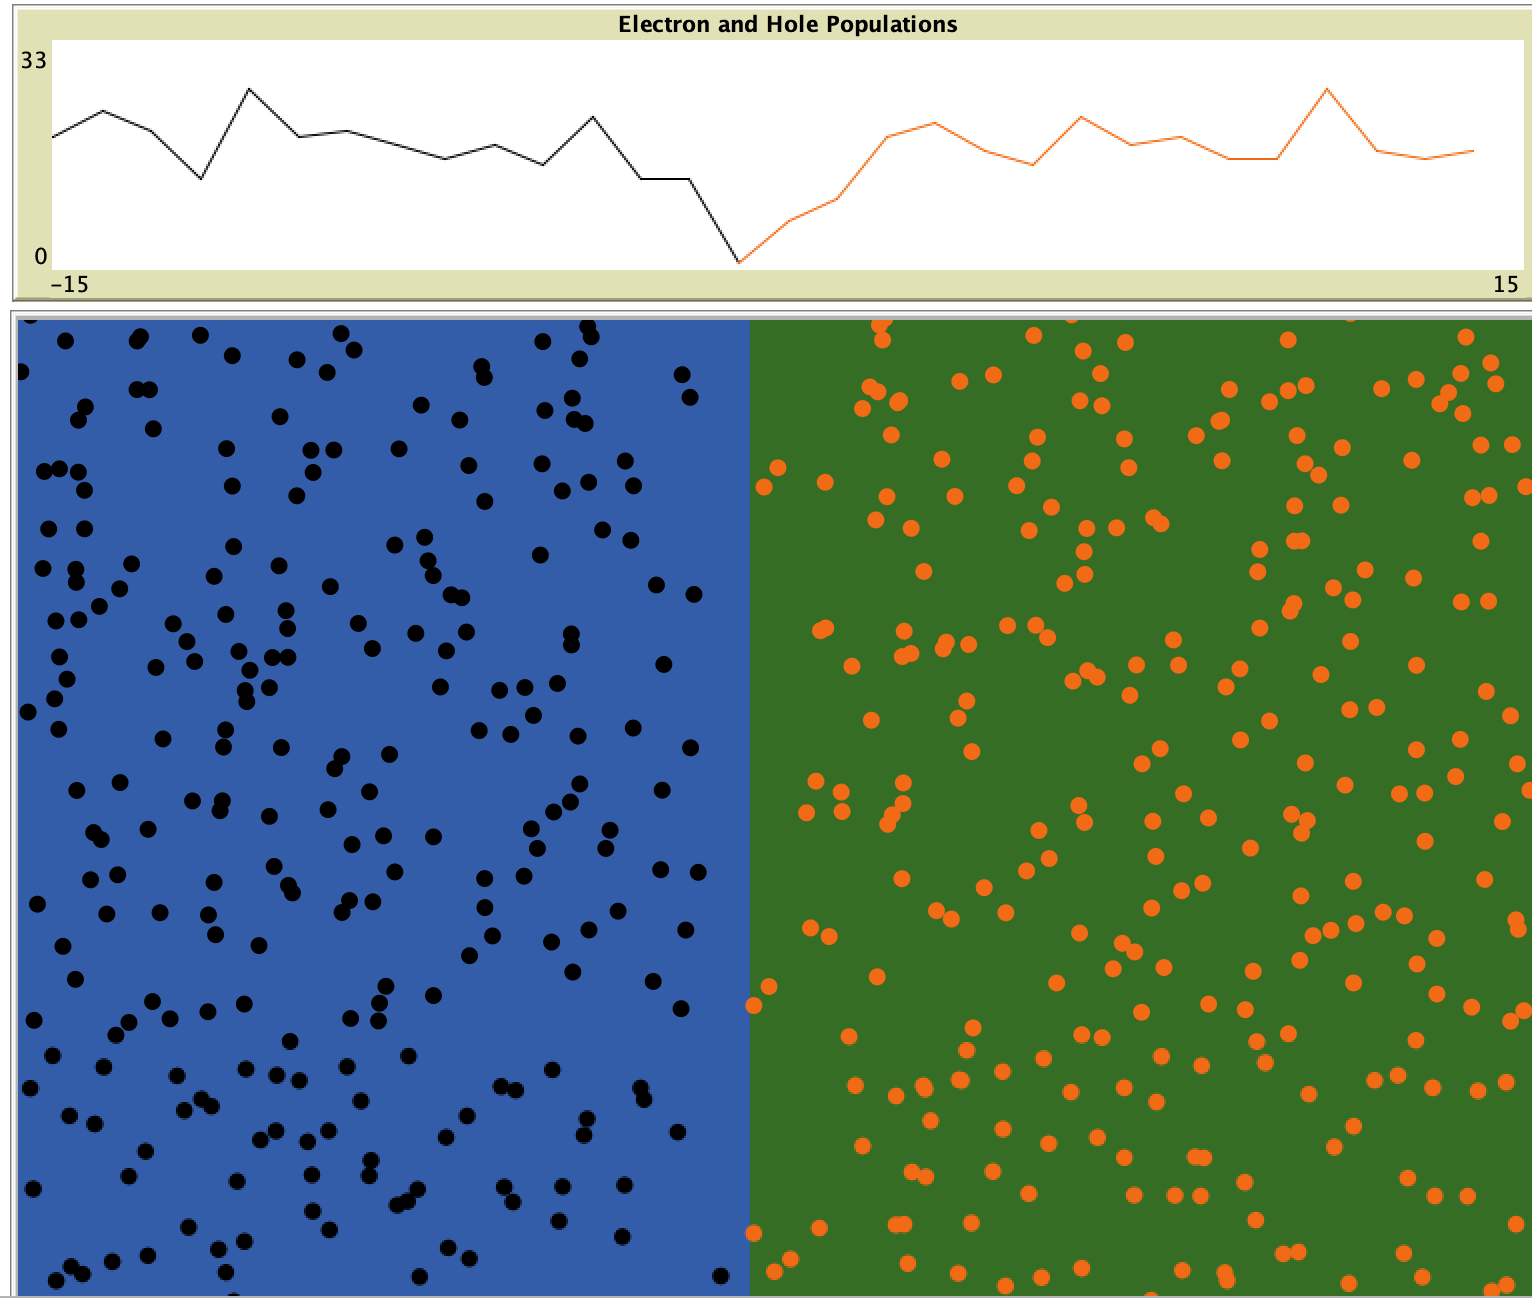
\includegraphics[width=0.8\columnwidth]{Figures/ModelSnapshot-2019-07-24}
\end{center}


\section{Model Assumptions}
\begin{itemize}
    \item Test.
\end{itemize}

\section{Model Limitations}

\begin{itemize}
    \item [v2019-07-24] Recombination probabilities are assumed to be 100\% --- electrons and holes do not produce recombination products --- making it impossible to model LEDs, PV, or other such devices.
    \item [v2019-07-24] Electrons and holes do not occupy positions within the band energy diagram and possess no energies.
    \item [v2019-07-24] The Monte Carlo algorithm treats the charge carriers as classical entities that will jump based on local field gradients. Contributions to the local fields include electron, hole, and ionic contributions.
    \item [v2019-07-24] We haven't yet included an applied field to drive drift.
    \item [v2019-07-24] We'll need to ultimately get a current across the junction. Currently, I'd expect that the recombination rate will be so high that few charge carriers will successfully cross the device.
    \item [v2019-07-24] How to model metal-semiconductor contacts?
    \item [v2019-07-24] What do we do for boundary conditions? Currently, just bounces off the boundary (high impedance).
\end{itemize}

\section{Possible Questions/Student Discovery}

\begin{itemize}
    \item (First predict)  and then construct plots in \textsection6.1.1.
    \item Adapt materials properties (substitute $n$- and $p$-type semiconductors, dopant concentrations, modify electron and hole mobilities).
    \item Discover rectifying behavior, MOSFET behavior, LED, PV.
    \item Can they sketch out band diagram from the observations they see with the formation of the depletion regime.
    \item Should be able to calculate the equilibrium depletion width and voltage... or at least derive the relationships between charge carrier concentration ($n_{n0}$) and voltage $V_0$.
\end{itemize}

It will model the emergence of the depletion regime as a consequence of charge recombination at the $p$-$n$ interface. Correlations between the agent-based model and \textit{in operando} behavior of ideal $p$-$n$ junctions,

MOSFETs, JFETs, LEDs and PV are possible. Prediction of $p$-$i$-$n$ diodes and rectifiers/amplifiers should also be possible (connect).

\section{Model issues/limitations.}
\begin{itemize}
    \item Our approach is to calculate the local fields to compute the charge carrier drift. Is this right?
    \item There are discontinuities in the plots of potential and $\mathcal{E}$-field. Is this simply 
\end{itemize}


\newpage
\printbibliography


\end{document}